\documentclass[final,a4paper,10pt,abstracton]{scrreprt}


\usepackage{draftwatermark}\SetWatermarkScale{5} %_DRAFT watermark

%
% General
\usepackage[english]{babel}
\usepackage{hyperref}
\hypersetup{final,plainpages=false,pagebackref,colorlinks=true,linkcolor=blue,urlcolor=red,citecolor=blue,pdfpagemode=UseOutlines,pdfstartview=FitH,pdfborder={0 0 0}}

\providecommand{\indexed}[1]{\index{#1}#1}

\newcommand{\HRule}{\rule{\linewidth}{0.5mm}}
\newcommand{\ie}{i.\,e.\ }
\newcommand{\eg}{e.\,g.\ }

%
% Graphics
\usepackage{pgfpages}
\usepackage{tikz}
\usetikzlibrary{arrows,positioning,shapes,topaths,calc,fit,backgrounds,matrix,shadows,automata}
\usepackage{soul}

%\usetikzlibrary{intersections}
%\usetikzlibrary{calc}
%\usetikzlibrary{positioning}


%
% Snippets 
\usepackage{moreverb}
\usepackage{listings}

% Tables
%-------------
\usepackage{tabularx}



\usepackage[underline=false,rounded corners=true]{macros/pgf-umlsd} % UML Sequence Diagrams macro

\title{The CernVM Co-Pilot}
% \subtitle{Technical Report}
\author{Artem Harutyunyan}

\providecommand{\cernvmcopilot}{{\scshape CernVM Co-Pilot~}}
\providecommand{\copilot}{{\scshape Co-Pilot~}}
\providecommand{\cern}{{\scshape cern~}}
\providecommand{\cernvm}{{\scshape CernVM~}}

\providecommand{\todo}[1]{\textcolor{red}{#1}}
\definecolor {light-blue}{rgb}{230,244,255}

\usepackage[nottoc]{tocbibind}

\usepackage{makeidx}
\makeindex

\setcounter{secnumdepth}{4}
\setcounter{tocdepth}{4}

\begin{document}

\selectlanguage{english}
\renewcommand\today{March 2011}

\pagestyle{empty}
\begin{titlepage}
	\begin{addmargin}[-\oddsidemargin]{-\evensidemargin}
  		\newlength{\saveparindent}
		\setlength{\saveparindent}{\parindent}
		\setlength{\parindent}{0cm}

  		\sf
		\center
		\vspace*{-1cm}
		\mbox{
	  		\parbox{4cm}{
				\resizebox{4cm}{!}{\begin{pgfpicture}
\pgfpathmoveto{\pgfqpoint{5.858cm}{9.523cm}}
\pgfpathlineto{\pgfqpoint{16.845cm}{9.523cm}}
\pgfpathlineto{\pgfqpoint{16.845cm}{20.265cm}}
\pgfpathlineto{\pgfqpoint{5.858cm}{20.265cm}}
\pgfpathclose
\pgfusepath{clip}
\begin{pgfscope}
\begin{pgfscope}
\end{pgfscope}
\begin{pgfscope}
\pgfpathmoveto{\pgfqpoint{0cm}{0cm}}
\pgfpathlineto{\pgfqpoint{21cm}{0cm}}
\pgfpathlineto{\pgfqpoint{21cm}{29.7cm}}
\pgfpathlineto{\pgfqpoint{0cm}{29.7cm}}
\pgfpathclose
\pgfusepath{clip}
\definecolor{eps2pgf_color}{rgb}{0.121569,0.337255,0.984314}\pgfsetstrokecolor{eps2pgf_color}\pgfsetfillcolor{eps2pgf_color}
\pgfpathmoveto{\pgfqpoint{8.912cm}{15.808cm}}
\pgfpathcurveto{\pgfqpoint{8.761cm}{15.793cm}}{\pgfqpoint{8.49cm}{15.793cm}}{\pgfqpoint{8.339cm}{15.793cm}}
\pgfpathlineto{\pgfqpoint{8.339cm}{16.471cm}}
\pgfpathlineto{\pgfqpoint{8.851cm}{16.471cm}}
\pgfpathcurveto{\pgfqpoint{8.927cm}{16.471cm}}{\pgfqpoint{9.002cm}{16.456cm}}{\pgfqpoint{9.078cm}{16.456cm}}
\pgfpathcurveto{\pgfqpoint{9.078cm}{16.471cm}}{\pgfqpoint{9.063cm}{16.502cm}}{\pgfqpoint{9.063cm}{16.517cm}}
\pgfpathcurveto{\pgfqpoint{9.063cm}{16.532cm}}{\pgfqpoint{9.078cm}{16.562cm}}{\pgfqpoint{9.078cm}{16.577cm}}
\pgfpathcurveto{\pgfqpoint{9.002cm}{16.577cm}}{\pgfqpoint{8.927cm}{16.562cm}}{\pgfqpoint{8.851cm}{16.562cm}}
\pgfpathlineto{\pgfqpoint{8.339cm}{16.562cm}}
\pgfpathlineto{\pgfqpoint{8.339cm}{17.15cm}}
\pgfpathlineto{\pgfqpoint{8.655cm}{17.15cm}}
\pgfpathlineto{\pgfqpoint{8.912cm}{17.135cm}}
\pgfpathcurveto{\pgfqpoint{8.987cm}{17.135cm}}{\pgfqpoint{9.063cm}{17.12cm}}{\pgfqpoint{9.138cm}{17.12cm}}
\pgfpathcurveto{\pgfqpoint{9.138cm}{17.135cm}}{\pgfqpoint{9.123cm}{17.165cm}}{\pgfqpoint{9.123cm}{17.18cm}}
\pgfpathcurveto{\pgfqpoint{9.123cm}{17.21cm}}{\pgfqpoint{9.138cm}{17.226cm}}{\pgfqpoint{9.138cm}{17.256cm}}
\pgfpathlineto{\pgfqpoint{8.113cm}{17.256cm}}
\pgfpathlineto{\pgfqpoint{8.113cm}{15.687cm}}
\pgfpathlineto{\pgfqpoint{9.153cm}{15.687cm}}
\pgfpathcurveto{\pgfqpoint{9.153cm}{15.702cm}}{\pgfqpoint{9.138cm}{15.732cm}}{\pgfqpoint{9.138cm}{15.748cm}}
\pgfpathcurveto{\pgfqpoint{9.138cm}{15.778cm}}{\pgfqpoint{9.153cm}{15.793cm}}{\pgfqpoint{9.153cm}{15.823cm}}
\pgfpathcurveto{\pgfqpoint{9.078cm}{15.808cm}}{\pgfqpoint{8.987cm}{15.808cm}}{\pgfqpoint{8.912cm}{15.808cm}}
\pgfpathmoveto{\pgfqpoint{11.023cm}{17.256cm}}
\pgfpathlineto{\pgfqpoint{10.933cm}{17.256cm}}
\pgfpathlineto{\pgfqpoint{10.933cm}{15.672cm}}
\pgfpathcurveto{\pgfqpoint{10.948cm}{15.687cm}}{\pgfqpoint{10.978cm}{15.687cm}}{\pgfqpoint{11.008cm}{15.687cm}}
\pgfpathcurveto{\pgfqpoint{11.023cm}{15.687cm}}{\pgfqpoint{11.053cm}{15.687cm}}{\pgfqpoint{11.068cm}{15.672cm}}
\pgfpathlineto{\pgfqpoint{11.068cm}{16.924cm}}
\pgfpathlineto{\pgfqpoint{11.099cm}{16.924cm}}
\pgfpathlineto{\pgfqpoint{12.199cm}{15.823cm}}
\pgfpathcurveto{\pgfqpoint{12.26cm}{15.763cm}}{\pgfqpoint{12.305cm}{15.717cm}}{\pgfqpoint{12.335cm}{15.672cm}}
\pgfpathlineto{\pgfqpoint{12.411cm}{15.672cm}}
\pgfpathlineto{\pgfqpoint{12.411cm}{17.256cm}}
\pgfpathcurveto{\pgfqpoint{12.38cm}{17.256cm}}{\pgfqpoint{12.365cm}{17.241cm}}{\pgfqpoint{12.335cm}{17.241cm}}
\pgfpathcurveto{\pgfqpoint{12.305cm}{17.241cm}}{\pgfqpoint{12.29cm}{17.256cm}}{\pgfqpoint{12.26cm}{17.256cm}}
\pgfpathlineto{\pgfqpoint{12.26cm}{16.064cm}}
\pgfpathlineto{\pgfqpoint{12.245cm}{16.064cm}}
\pgfpathclose
\pgfpathmoveto{\pgfqpoint{7.871cm}{15.928cm}}
\pgfpathcurveto{\pgfqpoint{7.826cm}{15.883cm}}{\pgfqpoint{7.615cm}{15.748cm}}{\pgfqpoint{7.328cm}{15.748cm}}
\pgfpathcurveto{\pgfqpoint{6.936cm}{15.748cm}}{\pgfqpoint{6.65cm}{16.019cm}}{\pgfqpoint{6.65cm}{16.471cm}}
\pgfpathcurveto{\pgfqpoint{6.65cm}{16.848cm}}{\pgfqpoint{6.876cm}{17.195cm}}{\pgfqpoint{7.343cm}{17.195cm}}
\pgfpathcurveto{\pgfqpoint{7.615cm}{17.195cm}}{\pgfqpoint{7.796cm}{17.045cm}}{\pgfqpoint{7.841cm}{16.999cm}}
\pgfpathlineto{\pgfqpoint{7.856cm}{16.999cm}}
\pgfpathcurveto{\pgfqpoint{7.871cm}{17.06cm}}{\pgfqpoint{7.886cm}{17.12cm}}{\pgfqpoint{7.901cm}{17.18cm}}
\pgfpathcurveto{\pgfqpoint{7.735cm}{17.241cm}}{\pgfqpoint{7.539cm}{17.286cm}}{\pgfqpoint{7.358cm}{17.286cm}}
\pgfpathcurveto{\pgfqpoint{6.815cm}{17.286cm}}{\pgfqpoint{6.393cm}{16.984cm}}{\pgfqpoint{6.393cm}{16.471cm}}
\pgfpathcurveto{\pgfqpoint{6.393cm}{15.974cm}}{\pgfqpoint{6.74cm}{15.657cm}}{\pgfqpoint{7.298cm}{15.657cm}}
\pgfpathcurveto{\pgfqpoint{7.494cm}{15.657cm}}{\pgfqpoint{7.705cm}{15.687cm}}{\pgfqpoint{7.856cm}{15.778cm}}
\pgfpathclose
\pgfpathmoveto{\pgfqpoint{9.605cm}{16.532cm}}
\pgfpathlineto{\pgfqpoint{9.605cm}{17.165cm}}
\pgfpathcurveto{\pgfqpoint{9.711cm}{17.165cm}}{\pgfqpoint{9.998cm}{17.18cm}}{\pgfqpoint{10.088cm}{17.165cm}}
\pgfpathcurveto{\pgfqpoint{10.284cm}{17.135cm}}{\pgfqpoint{10.375cm}{17.03cm}}{\pgfqpoint{10.375cm}{16.879cm}}
\pgfpathcurveto{\pgfqpoint{10.375cm}{16.698cm}}{\pgfqpoint{10.239cm}{16.577cm}}{\pgfqpoint{10.043cm}{16.547cm}}
\pgfpathcurveto{\pgfqpoint{9.922cm}{16.517cm}}{\pgfqpoint{9.651cm}{16.532cm}}{\pgfqpoint{9.605cm}{16.532cm}}
\pgfpathmoveto{\pgfqpoint{10.616cm}{15.868cm}}
\pgfpathlineto{\pgfqpoint{10.088cm}{16.471cm}}
\pgfpathcurveto{\pgfqpoint{10.344cm}{16.502cm}}{\pgfqpoint{10.616cm}{16.637cm}}{\pgfqpoint{10.616cm}{16.909cm}}
\pgfpathcurveto{\pgfqpoint{10.616cm}{17.135cm}}{\pgfqpoint{10.435cm}{17.256cm}}{\pgfqpoint{10.043cm}{17.256cm}}
\pgfpathlineto{\pgfqpoint{9.394cm}{17.256cm}}
\pgfpathlineto{\pgfqpoint{9.394cm}{15.672cm}}
\pgfpathcurveto{\pgfqpoint{9.44cm}{15.687cm}}{\pgfqpoint{9.47cm}{15.687cm}}{\pgfqpoint{9.515cm}{15.687cm}}
\pgfpathcurveto{\pgfqpoint{9.545cm}{15.687cm}}{\pgfqpoint{9.59cm}{15.687cm}}{\pgfqpoint{9.621cm}{15.672cm}}
\pgfpathlineto{\pgfqpoint{9.621cm}{16.441cm}}
\pgfpathlineto{\pgfqpoint{9.832cm}{16.441cm}}
\pgfpathlineto{\pgfqpoint{10.028cm}{16.23cm}}
\pgfpathlineto{\pgfqpoint{10.329cm}{15.883cm}}
\pgfpathcurveto{\pgfqpoint{10.39cm}{15.808cm}}{\pgfqpoint{10.435cm}{15.748cm}}{\pgfqpoint{10.495cm}{15.672cm}}
\pgfpathcurveto{\pgfqpoint{10.54cm}{15.687cm}}{\pgfqpoint{10.586cm}{15.687cm}}{\pgfqpoint{10.646cm}{15.687cm}}
\pgfpathcurveto{\pgfqpoint{10.691cm}{15.687cm}}{\pgfqpoint{10.736cm}{15.687cm}}{\pgfqpoint{10.782cm}{15.672cm}}
\pgfpathlineto{\pgfqpoint{10.736cm}{15.732cm}}
\pgfpathclose
\pgfpathmoveto{\pgfqpoint{9.163cm}{12.394cm}}
\pgfpathcurveto{\pgfqpoint{8.998cm}{12.418cm}}{\pgfqpoint{8.836cm}{12.452cm}}{\pgfqpoint{8.677cm}{12.496cm}}
\pgfpathcurveto{\pgfqpoint{9.079cm}{12.099cm}}{\pgfqpoint{9.564cm}{11.791cm}}{\pgfqpoint{10.102cm}{11.601cm}}
\pgfpathlineto{\pgfqpoint{10.285cm}{11.802cm}}
\pgfpathcurveto{\pgfqpoint{9.877cm}{11.933cm}}{\pgfqpoint{9.497cm}{12.134cm}}{\pgfqpoint{9.163cm}{12.394cm}}
\pgfpathmoveto{\pgfqpoint{8.327cm}{17.627cm}}
\pgfpathlineto{\pgfqpoint{8.641cm}{17.624cm}}
\pgfpathcurveto{\pgfqpoint{9.035cm}{18.135cm}}{\pgfqpoint{10.046cm}{18.893cm}}{\pgfqpoint{11.403cm}{18.893cm}}
\pgfpathcurveto{\pgfqpoint{11.698cm}{18.893cm}}{\pgfqpoint{11.985cm}{18.857cm}}{\pgfqpoint{12.259cm}{18.79cm}}
\pgfpathcurveto{\pgfqpoint{12.152cm}{18.903cm}}{\pgfqpoint{12.036cm}{19.008cm}}{\pgfqpoint{11.914cm}{19.106cm}}
\pgfpathcurveto{\pgfqpoint{11.747cm}{19.128cm}}{\pgfqpoint{11.576cm}{19.141cm}}{\pgfqpoint{11.403cm}{19.141cm}}
\pgfpathcurveto{\pgfqpoint{10.19cm}{19.141cm}}{\pgfqpoint{9.068cm}{18.589cm}}{\pgfqpoint{8.327cm}{17.627cm}}
\pgfpathmoveto{\pgfqpoint{11.403cm}{11.624cm}}
\pgfpathcurveto{\pgfqpoint{11.229cm}{11.624cm}}{\pgfqpoint{11.059cm}{11.639cm}}{\pgfqpoint{10.891cm}{11.663cm}}
\pgfpathlineto{\pgfqpoint{10.691cm}{11.444cm}}
\pgfpathcurveto{\pgfqpoint{10.923cm}{11.401cm}}{\pgfqpoint{11.161cm}{11.377cm}}{\pgfqpoint{11.403cm}{11.377cm}}
\pgfpathcurveto{\pgfqpoint{12.506cm}{11.377cm}}{\pgfqpoint{13.503cm}{11.84cm}}{\pgfqpoint{14.21cm}{12.581cm}}
\pgfpathlineto{\pgfqpoint{14.142cm}{12.873cm}}
\pgfpathcurveto{\pgfqpoint{13.475cm}{12.109cm}}{\pgfqpoint{12.495cm}{11.624cm}}{\pgfqpoint{11.403cm}{11.624cm}}
\pgfpathmoveto{\pgfqpoint{14.64cm}{13.119cm}}
\pgfpathcurveto{\pgfqpoint{14.956cm}{13.596cm}}{\pgfqpoint{15.169cm}{14.147cm}}{\pgfqpoint{15.248cm}{14.738cm}}
\pgfpathlineto{\pgfqpoint{15.265cm}{14.736cm}}
\pgfpathlineto{\pgfqpoint{15.889cm}{19.191cm}}
\pgfpathlineto{\pgfqpoint{15.643cm}{19.226cm}}
\pgfpathlineto{\pgfqpoint{15.2cm}{16.058cm}}
\pgfpathcurveto{\pgfqpoint{14.939cm}{17.301cm}}{\pgfqpoint{14.082cm}{18.327cm}}{\pgfqpoint{12.942cm}{18.822cm}}
\pgfpathcurveto{\pgfqpoint{13.044cm}{18.688cm}}{\pgfqpoint{13.138cm}{18.548cm}}{\pgfqpoint{13.223cm}{18.403cm}}
\pgfpathcurveto{\pgfqpoint{14.307cm}{17.773cm}}{\pgfqpoint{15.038cm}{16.6cm}}{\pgfqpoint{15.038cm}{15.259cm}}
\pgfpathcurveto{\pgfqpoint{15.038cm}{14.605cm}}{\pgfqpoint{14.863cm}{13.992cm}}{\pgfqpoint{14.56cm}{13.462cm}}
\pgfpathclose
\pgfpathmoveto{\pgfqpoint{7.769cm}{15.259cm}}
\pgfpathlineto{\pgfqpoint{7.77cm}{15.344cm}}
\pgfpathlineto{\pgfqpoint{7.522cm}{15.35cm}}
\pgfpathlineto{\pgfqpoint{7.521cm}{15.259cm}}
\pgfpathcurveto{\pgfqpoint{7.521cm}{14.938cm}}{\pgfqpoint{7.56cm}{14.619cm}}{\pgfqpoint{7.638cm}{14.31cm}}
\pgfpathcurveto{\pgfqpoint{7.724cm}{13.965cm}}{\pgfqpoint{7.857cm}{13.642cm}}{\pgfqpoint{8.026cm}{13.344cm}}
\pgfpathcurveto{\pgfqpoint{8.161cm}{13.268cm}}{\pgfqpoint{8.303cm}{13.202cm}}{\pgfqpoint{8.448cm}{13.143cm}}
\pgfpathcurveto{\pgfqpoint{8.189cm}{13.506cm}}{\pgfqpoint{7.992cm}{13.918cm}}{\pgfqpoint{7.878cm}{14.371cm}}
\pgfpathcurveto{\pgfqpoint{7.805cm}{14.659cm}}{\pgfqpoint{7.769cm}{14.958cm}}{\pgfqpoint{7.769cm}{15.259cm}}
\pgfpathmoveto{\pgfqpoint{13.376cm}{16.381cm}}
\pgfpathcurveto{\pgfqpoint{13.376cm}{14.377cm}}{\pgfqpoint{11.745cm}{12.747cm}}{\pgfqpoint{9.741cm}{12.747cm}}
\pgfpathcurveto{\pgfqpoint{8.072cm}{12.747cm}}{\pgfqpoint{6.622cm}{13.876cm}}{\pgfqpoint{6.216cm}{15.493cm}}
\pgfpathcurveto{\pgfqpoint{6.144cm}{15.782cm}}{\pgfqpoint{6.107cm}{16.081cm}}{\pgfqpoint{6.107cm}{16.381cm}}
\pgfpathcurveto{\pgfqpoint{6.107cm}{18.385cm}}{\pgfqpoint{7.737cm}{20.016cm}}{\pgfqpoint{9.741cm}{20.016cm}}
\pgfpathcurveto{\pgfqpoint{11.745cm}{20.016cm}}{\pgfqpoint{13.376cm}{18.385cm}}{\pgfqpoint{13.376cm}{16.381cm}}
\pgfpathmoveto{\pgfqpoint{9.741cm}{20.263cm}}
\pgfpathcurveto{\pgfqpoint{7.601cm}{20.263cm}}{\pgfqpoint{5.859cm}{18.522cm}}{\pgfqpoint{5.859cm}{16.381cm}}
\pgfpathcurveto{\pgfqpoint{5.859cm}{16.06cm}}{\pgfqpoint{5.899cm}{15.741cm}}{\pgfqpoint{5.976cm}{15.433cm}}
\pgfpathcurveto{\pgfqpoint{5.984cm}{15.4cm}}{\pgfqpoint{5.995cm}{15.369cm}}{\pgfqpoint{6.004cm}{15.337cm}}
\pgfpathlineto{\pgfqpoint{6.002cm}{15.336cm}}
\pgfpathlineto{\pgfqpoint{6.975cm}{11.854cm}}
\pgfpathlineto{\pgfqpoint{7.214cm}{11.92cm}}
\pgfpathlineto{\pgfqpoint{6.607cm}{14.092cm}}
\pgfpathcurveto{\pgfqpoint{7.321cm}{13.114cm}}{\pgfqpoint{8.47cm}{12.499cm}}{\pgfqpoint{9.741cm}{12.499cm}}
\pgfpathcurveto{\pgfqpoint{10.379cm}{12.499cm}}{\pgfqpoint{10.98cm}{12.654cm}}{\pgfqpoint{11.511cm}{12.928cm}}
\pgfpathlineto{\pgfqpoint{8.408cm}{9.525cm}}
\pgfpathlineto{\pgfqpoint{8.743cm}{9.525cm}}
\pgfpathlineto{\pgfqpoint{12.61cm}{13.765cm}}
\pgfpathlineto{\pgfqpoint{12.608cm}{13.767cm}}
\pgfpathcurveto{\pgfqpoint{13.132cm}{14.341cm}}{\pgfqpoint{13.486cm}{15.073cm}}{\pgfqpoint{13.59cm}{15.882cm}}
\pgfpathlineto{\pgfqpoint{15.075cm}{9.525cm}}
\pgfpathlineto{\pgfqpoint{15.329cm}{9.525cm}}
\pgfpathlineto{\pgfqpoint{13.521cm}{17.264cm}}
\pgfpathlineto{\pgfqpoint{13.521cm}{17.264cm}}
\pgfpathcurveto{\pgfqpoint{13.224cm}{18.532cm}}{\pgfqpoint{12.305cm}{19.564cm}}{\pgfqpoint{11.104cm}{20.016cm}}
\pgfpathlineto{\pgfqpoint{16.843cm}{20.016cm}}
\pgfpathlineto{\pgfqpoint{16.843cm}{20.263cm}}
\pgfusepath{fill}
\end{pgfscope}
\end{pgfscope}
\end{pgfpicture}}
%				
%				%\begin{tikzpicture}[scale=0.5]
%				%	\path[fill=black, join=round] (1,1)--(2,2)--(2,5)--(5,5)--(6,6)--(1,6)--(1,1)--(2,0)--(5,0)--(7,2)--(7,5)--(6,6)--(6,1)--cycle;
%				%	\clip (6,6)--(5,5)--(5,2)--(2,2)--(1,1)--(6,1)--(6,6)--(5,7)--(2,7)--(0,5)--(0,2)--(1,1)--(1,6)--cycle;
%				%	\shade[inner color=green, outer color=black] (3,4) circle(5.5cm);
%				%\end{tikzpicture}
	  		}
	  		\parbox{9cm}{
	    			%\LARGE CERN\\
	    			%\large PH-SFT%\\[0.5cm]
			}
		}
		\vspace*{2.5cm}
 
  		{\large \scshape Portable Analysis Environment using Virtualization Technology (WP9)}\\[0.5cm]
  		\HRule\\[0.4cm]
		\huge Co-Pilot: The Distributed Job Execution Framework\\
		\HRule\\[1.5cm]
		
%        \includegraphics[height=5cm]{marbles}\\[1.5cm]
        
\includegraphics{img/IMG_cernvmlogo}\\[1.5cm] 
		\large Predrag Buncic \qquad Artem Harutyunyan\\[0.4cm]
		%\today
  
  		\vfill
		\large Refers to Co-Pilot 0.1\\[1ex]
		%  \LARGE ---DRAFT---\\[1ex]
		%  \LARGE www.grgen.net\\[6ex]
		%  \LARGE Jakob Blomer \qquad Rubino Gei\ss\\[3ex]
		%  \large \today\\
  
		\vfill
		\large Technical Report\\
		Version: 0.1 (Draft) \today 
		%	\large ISSN 1432-7864	

  		\setlength{\parindent}{\saveparindent}
	\end{addmargin}
\end{titlepage}
\cleardoublepage
\pagenumbering{roman}



\abstract{
The \cernvmcopilot\ is a framework which allows to integrate cloud and volunteer computing resources into the existing Grid infrastructures and exploit those resources for the execution of Grid jobs.  
It can also be used to instantiate an independent ad-hoc distributed computing infrastructure  on top of virtualized resources.  
}

\tableofcontents
\clearpage
\pagenumbering{arabic}
\pagestyle{headings}

\chapter{Overview}
\label{sct:overview}

The job execution in Grid infrastructures of LHC experiments is done using so-called \indexed{pilot job} approach: experiments come into posession 
of Grid resrouces using special kind of jobs, known as '\indexed{pilot job}s' (or 'job agents', 'pilot agents', 'pilots'), after which they use their 
own job submission and scheduling systems (e.g. \cite{alien, dirac, panda, crab} ) to deliver and execute Grid users' jobs on those resources. 

After landing on the worker nodes of the computing sites the \indexed{pilot job}s inspect the machine configuration (e.g. check which software packages 
are available), make necessary preparations for the execution of the real job (e.g. install experiment application packages), report to the experiment 
scheduling system the configuration of the machine (e.g. available disk space and memory), fetch the real job for execution, fork a process and start 
execution of the real job within that process. 

\cernvmcopilot\ is a framework for execution of LHC experiments' \indexed{pilot job}s on a wide choice of extra (and so far untapped by 
LHC experiments) computing resources such as enterprise cloud computing infrastructures (e.g. Amazon EC2 \cite{ec2}), scientific computing 
clouds (e.g. Nimbus \cite{nimbus, scienceClouds} ), and, last but not least, cloud of BOINC (\cite{boinc}) volunteer PC's. \copilot\ serves 
as a gateway between differing \indexed{pilot job} implementations of the LHC experiments and cloud resources. On each experiment's side of 
the gateway so-called \copilot\ Adapter service is required. Currently such adapers have been developed for both ALICE and ATLAS, adapters 
for CMS and LHCb should be produced in order to complete the system.

In order to provide additional computing resources to the LHC experiments, it is important not to expect the physicists who run job production to 
make changes to their existing scripts or procedures, that is why the \copilot\ is designed in a way that the integration of the external 
resources is completely transparent for end-users.

All the code needed to support the \copilot\ services and to communicate with the Grid services of experiments is included in 
the \cernvm\ \cite{cernvm08, cernvmWeb} images that we use. The images also contain the ready-to-use LHC experiments' 
application frameworks.

The \copilot\ framework (Figure~\ref{fig:architecture}) consists of the \indexed{\copilot\ Agent} � a lightweight program which runs inside virtual 
machines deployed on the cloud, and of \indexed{\copilot\ Service}s -- components which orchestrate the work of \copilot
\ Agents. Agents and Services communicate by means of Jabber/XMPP \cite{rfc3920,rfc3921} instant messaging network using a 
specially developed protocol. The \copilot\ Service components are stateless which in conjunction with the use of Jabber/XMPP allows 
to scale the system in case of high load by just deploying new Service instances and adding them to the existing messaging network .  

Co-Pilot framework has two goals. The first goal is to integrate cloud resources with the existing grid infrastructures by seamlessly extending experiment grid pilot job frameworks. The second goal is to provide a toolkit which can be used to quickly instantiate an ad-hoc distributed computing infrastructure on top of cloud resources. Such a need often arises within the relatively small experiments or research groups (e.g. NA61 experiment~\cite{laszlo2009na61}, CERN Theoretical Physics group) which do not have enough resources to deploy and maintain a grid infrastructure. 


\begin{figure}
	\begin{center}
		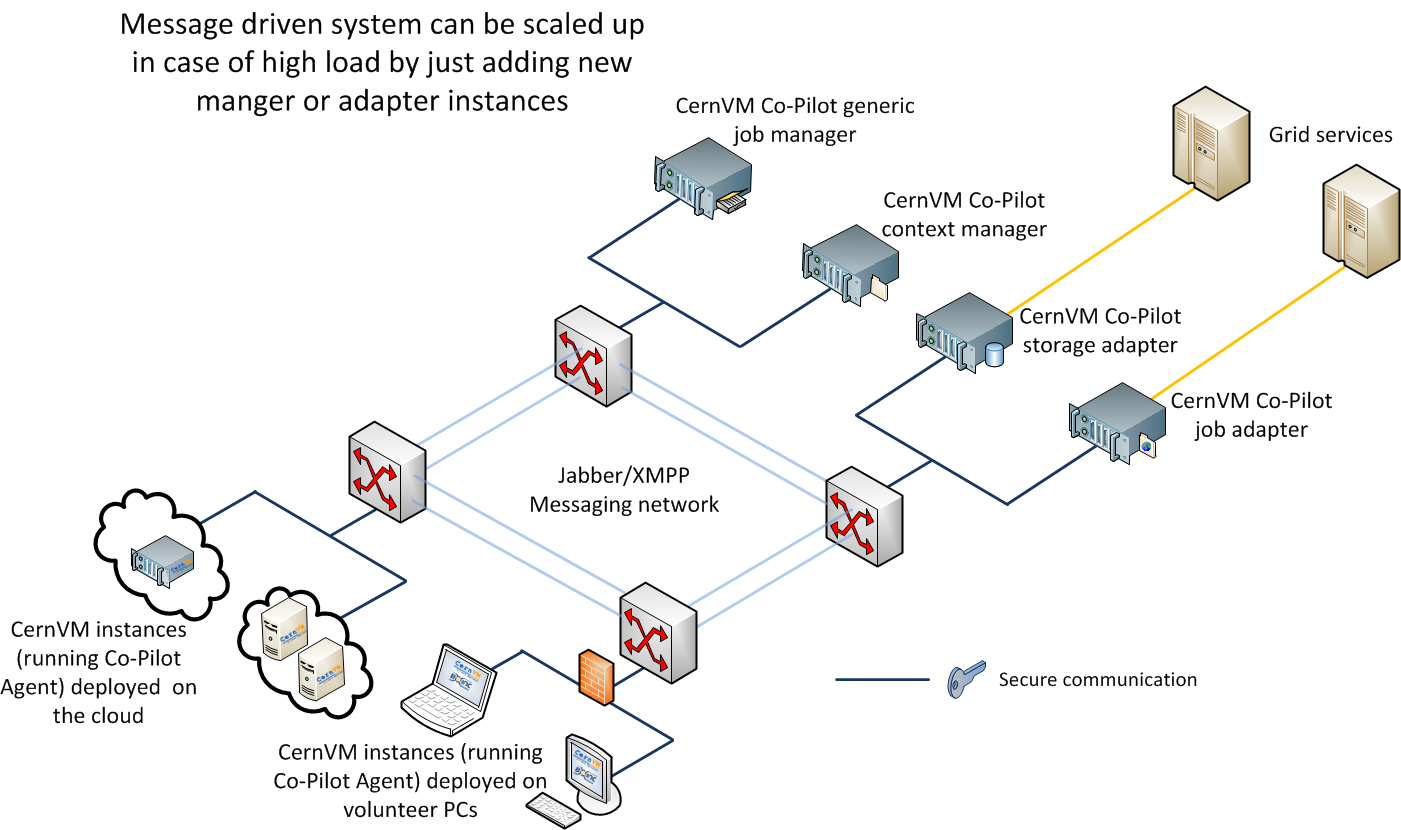
\includegraphics[scale=0.2]{img/IMG_Co-Pilot_Architecture.png}
	\end{center}
	\caption{The architecture of \cernvmcopilot framework}
	\label{fig:architecture}
\end{figure}

The components of the \copilot~framework are listed in Table~\ref{tbl:components}. 

\begin{table}
  \begin{center}

    \begin{tabularx}{\linewidth}{l|X}
      {\bf\centering \copilot component name} & {\bf\centering Description} \\\hline
        \texttt{Agent} & Communicates with service insances and requests a job to execute. Upon receiving the job downloads the input 
                         files, executes the job, uploads job output files and reports that the job execution is finished. \\
        \texttt{Generic Job and Storage Manager} & Distributes jobs from the internal queue to Agents for execution, provides space for storing 
                                                   the job output   \\
        \texttt{AliEn Job Manager} & Retrieves jobs from the central task queue of \indexed{AliEn} Grid \cite{alien} and sends them to 
                                     Agents for execution \\
        \texttt{AliEn Storage Manager} & Uploads the output of AliEn jobs executed by Agents and finalizes the job status in AliEn Grid.  \\
        \texttt{PanDA Storage Manager} & Uploads the output of \indexed{PanDA} \cite{panda} jobs executed by Agents and finalizes the job status in PanDA Grid  \\
    \end{tabularx}  
  \end{center}

  \caption{List of \copilot componentns}

  \label{tbl:components}
\end{table}



\chapter{\cernvmcopilot Internals}
\label{sct:protocol}

\section{Introduction}
Agents communicate with services over Jabber/XMPP \cite{rfc3920,rfc3921} instant messaging protocol. The messages they
exchange are formatted using XML. The messages are enclosed in \emph{$<$message$>$} tag, which has three attributes: \emph{'from'} and
\emph{'to'} (sender's and receiver's Jabber IDs), as well as the \emph{'id'} tag (unique ID of the message). The content of the message is enclosed in \emph{$<$body$>$} tag. All the values inside \emph{$<$body$>$} are
base64 \cite{rfc3548} encoded.

Each message body contains the \emph{'info'} tag. \emph{'info'} has the \emph{'command'} attribute, which contains the command needed
to be performed by the peer (e.g. Agent sends 'jobDone' command when it has finished executing the job and uploading files). The \emph{'info'} tag also contains other attributes necessary to perform the command. Below we present the list of commands which agents send along with the appropriate response commands which they expect in response. 

Every message by default should be acknowledged by the recipient by sending the \emph{ack} message, with empty \emph{'body'} tag. The ID of the message being acknowledged is set as the value of \emph{'ack'} attribute.
Example:

\lstset{backgroundcolor=\color{light-blue}}
\lstset{tabsize=2, basicstyle=\footnotesize, captionpos=b}
\lstset{caption=Example \emph{'ack'} message, label=fig:ack}
\lstset{frame=single, language=XML}
\begin{lstlisting}
<message to='jm@jabber.org'
                    from='agent@jabber.org'
                    ack='1a58119b-5c0e-47e8-8320-b865cc4a502e'
                    >
                   <body>  </body>
</message>
\end{lstlisting}

Acknowledgements can be disabled for arbitrary messages by including a \emph{'noack'} property in the \emph{'message'} tag.
This property will signal the recipient not to send an acknowledgement.
Example:

\lstset{backgroundcolor=\color{light-blue}}
\lstset{tabsize=2, basicstyle=\footnotesize, captionpos=b}
\lstset{caption=Example message , label=fig:noack}
\lstset{frame=single, language=XML}
\begin{lstlisting}
<message to='mon@jabber.org'
         from='jm@jabber.org/alpha'
         noack='1'>
         <body>
            <info command='__BASE64:cmVwb3J0RXZlbnQ='
                  component='__BASE64:am9ib...scGhh'
                  event='__BASE64:c2Vzc2lvbi5zdGFydA=='/>
         </body>
</message>
\end{lstlisting}

\section{Protocol commands}

\subsection{Job request}
\label{sct:protojobrequest}

When Agent has a slot for running a job it broadcasts to the Job Managers the \emph{'\indexed{want\_getJob}'} (sect. ~\ref{sct:wantgetjob})
request which contains Agent's configuration formatted in JDL \cite{jdl}, hostname and the \textcolor{red}{ip (to be implemented)}
of the machine where the Agent runs. Upon receiving the message job managers which have jobs for execution send back to
the agent \emph{'\indexed{have\_getJob}'} \ref{sct:havegetjob} command. The agent makes actual job request (\emph{'\indexed{getJob}'} command \ref{sct:getjob})
to the job manager from which the first \emph{'\indexed{have\_getJob}'} \ref{sct:havegetjob} command has been received. The job manager replies with
\emph{'\indexed{runJob}'} \ref{sct:runjob} command which contains the information about the job. The job request sequence is presented on
Figure~\ref{fig:jobreq}. Below the format of the job request commands is described.

\begin{figure}
  \centering

  \begin{sequencediagram}
    \tikzstyle{instyle}+=[rounded corners=3.2mm, bottom color=blue]
      \newthread{agent}{Co-Pilot Agent}
      \newinstmult[5]{manager}{Co-Pilot Job Manager}

      \begin{call}{agent}{want\_getJob}{manager}{have\_getJob}
      \end{call}

      \begin{call}{agent}{getJob}{manager}{runJob}
      \end{call}
  \end{sequencediagram}
  \caption{Job request commands}
  \label{fig:jobreq}
\end{figure}

\subsubsection{\indexed{want\_getJob}}
\label{sct:wantgetjob}
This message is used to chose a Job Manager to which a \emph{'\indexed{getJob}'} request \ref{sct:getjob} request eventually is
going to be made: the client sends it to the broadcast address and continues the communication with the Job Manager from which responded the quickest.
\emph{\bf $<$info$>$ tag attributes and their values}
\begin{itemize}
  \item \emph{command} - 'want\_getJob'
  \item \emph{agentHost} - hostname of the agent
  \item \todo{\emph{agentIP} - ip of the agent' to be implemented}
  \item \emph{jdl - agent host configuration in JDL format}
\end{itemize}

Example:

\lstset{backgroundcolor=\color{light-blue}}
\lstset{tabsize=2, basicstyle=\footnotesize, captionpos=b}
\lstset{caption=Example \emph{'want\_getJob'} request, label=fig:wantgetjobexpl}
\lstset{frame=single, language=XML}
% \lstset{numbers=left, numberstyle=\tiny, stepnumber=2, numbersep=5pt}
% \lstset{keywordstyle=\color{red}\bfseries\emph}
\begin{lstlisting}
<message to='jm@jabber.org' from='agent@jabber.org'>
  <body>
    <info agentHost='_BASE64:Y3ZtYXBwaTI0LmNlcm4uY2g='
          jdl='_BASE64:CiAgICBbCi...........KICAgIF0='
          command='_BASE64:Z2V0Sm9i'
    />
  </body>
</message>
\end{lstlisting}

The host configuration in JDL format has the following attributes:

\lstset{backgroundcolor=\color{light-blue}}
\lstset{tabsize=2, basicstyle=\footnotesize, captionpos=b}
\lstset{caption=Example host configuration in JDL format, label=fig:wantgetjobexpl}
\lstset{frame=single}
\begin{lstlisting}
[
  Requirements = ( other.Type == "Job" );
  Version = "0";
  Platform = "Linux-i686";
  LocalDiskSpace = 4257288;
  WNHost = "cvmappi24.cern.ch";
  Memory = 1010;
  Type = "machine";
  Uname = "2.6.26.8-0.1.smp.gcc3.4.x86.i686";
  FreeMemory = 683;
  Swap = 127;
  FreeSwap = 127
]
\end{lstlisting}

\subsubsection{\indexed{have\_getJob}}
\label{sct:havegetjob}
This message is sent by the job manager as a reply to \emph{'\indexed{want\_getJob}'} \ref{sct:wantgetjob} message.

\emph{\bf $<$info$>$ tag attributes and their values}
\begin{itemize}
  \item \emph{command} - 'have\_getJob'
  \item \emph{requireFile} - prerequisite file (optional)
 \end{itemize}

Before making \emph{'\indexed{getJob}'} \ref{sct:getjob} request Agent has to make sure that a file required by \emph{requireFile} attribute is present on the host.
In case when attribute is not present in the message sent by the Job Manager no checks are necessary.

\subsubsection{\indexed{getJob}}
\label{sct:getjob}
Once the client knows the full JID (Jabber ID + resource) of the Job Manager which has a matching job it sends the real job request which (should eventually result in the  \emph{'\indexed{runJob}'} response \ref{sct:runjob}). The   \emph{'\indexed{getJob}'}  message should has the same format as \emph{'\indexed{want\_getJob}'}.

\emph{\bf $<$info$>$ tag attributes and their values}
\begin{itemize}
  \item \emph{command} - 'want\_getJob'
  \item \emph{agentHost} - hostname of the agent
  \item \todo{\emph{agentIP} - ip of the agent' to be implemented}
  \item \emph{jdl - agent host configuration in JDL format}
\end{itemize}


\subsubsection{\indexed{runJob}}
\label{sct:runjob}

Upon receiving \emph{'\indexed{getJob}'} \ref{sct:getjob} request from the client the Job Manager sends to the client the job for execution.

\emph{\bf $<$info$>$ tag attributes and their values}
\begin{itemize}
  \item \emph{command} - 'runJob'
  \item \emph{jmJobData} - Internal data describing the job (optional)
  \item \emph{job} - Job information is enclosed in $<$job$>$ tag, which contains the following attributes:
    \subitem \emph{chirpUrl} - Address of Chirp server from where to get the job input and put the job output (NOTE: Will be changed by the reference to storage adapter which the Agent should ask for the input and upload output)
    \subitem \emph{inputDir} - Directory on Chirp server from which to get the input files of the job
    \subitem \emph{environment} - Environment variables which must be set before job execution
    \subitem \emph{outputDir} - Directory to which to write the output
    \subitem \emph{packages} - List of application software packages needed by the job
    \subitem \emph{inputFiles} - List of job input files
    \subitem \emph{arguments} - Command line arguments of the job execution command
    \subitem \emph{id} - Job ID
    \subitem \emph{command} - Job execution command
    \subitem \emph{validation} - Name of the script for validating the job after it is finished (optional)
\end{itemize}

If the Job Manager sends the optional \emph{'jmJobData'} property, then the agent will re-send the same value in subsequent requests. If the property isn't provided, Agent will omit it as well.

\begin{figure}
  \centering
  \begin{sequencediagram}
    \tikzstyle{instyle}+=[rounded corners=3.2mm, bottom color=blue]
      \newthread{agent}{Co-Pilot Agent}
      \newinstmult[5]{manager}{Co-Pilot Job (or Storage) Manager}

      \begin{call}{agent}{want\_getJobOutputDir}{manager}{have\_getJobOutputDir}
      \end{call}
      \begin{call}{agent}{getJobOutputDir}{manager}{storeJobOutputDir}
      \end{call}

  \end{sequencediagram}
  \caption{Output directory request commands}
  \label{fig:outputdirreq}
\end{figure}

\subsection{Job output directory request}
\label{sct:joboutput}
When the job execution is finished the client asks the Storage Manager to provide a directory where the output produced by the job must be stored. The client sends a \emph{'\indexed{want\_getJobOutputDir}'} \ref{sct:wantgetjoboutputdir} request to choose the Job or Storage manager, which is followed by \emph{'\indexed{getJobOutputDir}'} request \ref{sct:getjoboutputdir}. The client expects  \emph{'\indexed{storeJobOutputDir}'} \ref{sct:storejoboutputdir} response. Output directory request sequence is given on Figure \ref{fig:outputdirreq}.

\subsubsection{\indexed{want\_getJobOutputDir}}
\label{sct:wantgetjoboutputdir}
This message is used to chose a Job Manager (or a Storage Manager) to which a \emph{'\indexed{getJobOutputDir}'} request \ref{sct:getjoboutputdir} request eventually is
going to be made: the client sends it to the broadcast address and continues the communication with the Job Manager (or a Storage Manager) from which responded the quickest.

\emph{\bf $<$info$>$ tag attributes and their values}
\begin{itemize}
  \item \emph{command} - 'want\_getJobOutputDir'
  \item \emph{agentHost} - Hostname of the client
  \item \todo{\emph{agentIP} - IP of the agent' to be implemented}
  \item \emph{jobID} - Job ID (the one which was received with runJob)
  \item \emph{jmJobData} - Internal data associated with the job (optional)
\end{itemize}

If the \emph{'jmJobData'} property was already sent to the Agent (with \emph{'runJob'} command), then the Agent will update its value and accordingly send the new value with subsequent requests.

\subsubsection{\indexed{have\_getJobOutputDir}}
\label{sct:havegetjoboutputdir}
This message is sent by the Job or Storage Manager as a reply to \emph{'\indexed{want\_getJobOutputDir}'} \ref{sct:wantgetjoboutputdir} message.

\emph{\bf $<$info$>$ tag attributes and their values}
\begin{itemize}
  \item \emph{command} - 'have\_getJobOutputDir'
 \end{itemize}

\subsubsection{\indexed{getJobOutputDir}}
\label{sct:getjoboutputdir}
Clients send the output job directory request to storage server when the job was executed and the output needs to be uploaded.

\emph{\bf $<$info$>$ tag attributes and their values}
\begin{itemize}
  \item \emph{command} - 'getJobOutputDir'
  \item \emph{agentHost} - Hostname of the client
  \item \emph{jobID} - Job ID (the one which was received with runJob)
  \item \emph{jmJobData} - Job Manager's internal data associated with the job
\end{itemize}

\subsubsection{\indexed{storeJobOutputDir}}
\label{sct:storejoboutputdir}
When Adapter receives an output directory request from the job it creates the directory, sets the write access permission to the Agent, and sends back the directory address.

\emph{\bf $<$info$>$ tag attributes and their values}
\begin{itemize}
  \item \emph{command} - 'storeJobOutputDir'
  \item \emph{outputChirpUrl} - Chirp server host and port (separated by semicolon)
  \item \emph{outputDir} - Directory on the chirp server to put files
  \item \emph{jobID} - Job ID (the one which was received with getJobOutputDir)
  \item \emph{jmJobData} - Job Manager's internal data associated with the job (optional)
\end{itemize}

\subsection{Job completion}
\subsubsection{\indexed{jobDone}}
\label{sct:jobdone}
When the job command execution is over and output files are uploaded to the output directory the client reports to the Job Manager that the job is done. Job completion request sequence is presented on Figure \ref{fig:jobdone}.
\begin{figure}
  \centering
  \begin{sequencediagram}
    \tikzstyle{instyle}+=[rounded corners=3.2mm, bottom color=blue]
      \newthread{agent}{Co-Pilot Agent}
      \newinstmult[5]{manager}{Co-Pilot Job Manager}
      \mess{agent}{jobDone}{manager}
  \end{sequencediagram}
  \caption{Job completion command}
  \label{fig:jobdone}
\end{figure}

\emph{\bf $<$info$>$ tag attributes and their values}
\begin{itemize}
  \item \emph{command} - 'jobDone'
  \item \emph{exitCode} - Job execution exit code
  \item \emph{agentHost} - Hostname of the client
  \item \emph{state} - Job state (e.g. 'done')
  \item \emph{jobID} - Job ID
  \item \emph{jmJobData} - Job Manager's internal data associated with the job
\end{itemize}

\subsection{Redirection of commands}

Messages exchanged by Co-Pilot components can be redirected. This allows having separate instances  of Managers for performing different tasks and in the same time configuring clients only with a single communication address. For example one can setup an adapter which is used to retrieve job details and input files and another adapter which is used to upload job execution results and does job finalization (e.g. the use case of ALICE experiment \ref{sct:usecasealice}).

\begin{figure}
  \centering
  \begin{sequencediagram}
    \tikzstyle{instyle}+=[rounded corners=3.2mm, bottom color=blue]
      \newthread{agent}{Co-Pilot Agent}
      \newinstmult[2]{manager}{Co-Pilot Manager}

      \begin{call}{agent}{want\_getJob}{manager}{redirect}
      \end{call}

      \newinst[1]{jobmanager}{Co-Pilot Job Manager}

      \begin{call}{agent}{want\_getJob}{jobmanager}{have\_getJob}
      \end{call}
  \end{sequencediagram}
  \caption{Job request commands}
  \label{fig:redirect}
\end{figure}


\subsubsection{\indexed{redirect}}
\label{sct:redirect}

\emph{\bf $<$info$>$ tag attributes and their values}
\begin{itemize}
  \item \emph{command} - 'redirect'
  \item \emph{referral} - Jabber ID of the service to which the redirection should be made
  \item \emph{info} - Data which should be conveyed to the referral
 \end{itemize}


Example:

The following redirection command received by the Co-Pilot component

\lstset{backgroundcolor=\color{light-blue}}
\lstset{tabsize=2, basicstyle=\footnotesize, captionpos=b}
\lstset{caption=Example \emph{'want\_getJob'} request, label=fig:redirect}
\lstset{frame=single, language=XML}
% \lstset{numbers=left, numberstyle=\tiny, stepnumber=2, numbersep=5pt}
% \lstset{keywordstyle=\color{red}\bfseries\emph}
\begin{lstlisting}
<message to='agent@cvmappi21.cern.ch' from='jmreal@cvmappi21.cern.ch'>
	<body>
		<info referral='_BASE64:c3RvcmFnZXJlYWxAY3ZtYXBwaTIxLmNlcm4uY2g='
	              command='_BASE64:cmVkaXJlY3Q='>
			<info to='_BASE64:am1yZWFsQGN2bWFwcGkyMS5jZXJuLmNo'
			      exitCode='_BASE64:MA=='
			      jobID='_BASE64:MzA4MDE3NDE='
			      state='_BASE64:ZG9uZQ=='
            jmJobData='_BASE64:c3RhcnRlZEF0PQo='
			      command='_BASE64:am9iRG9uZQ==' />
		</info>
	</body>
</message>
\end{lstlisting}

will result into sending the following message to 'storagereal@cvmappi21.cern.ch' (which corresponds to the Base64 decoded value of 'referral' attribute from previous command):

\lstset{backgroundcolor=\color{light-blue}}
\lstset{tabsize=2, basicstyle=\footnotesize, captionpos=b}
\lstset{caption=Example \emph{'want\_getJob'} request, label=fig:realredirectxml}
\lstset{frame=single, language=XML}
% \lstset{numbers=left, numberstyle=\tiny, stepnumber=2, numbersep=5pt}
% \lstset{keywordstyle=\color{red}\bfseries\emph}
\begin{lstlisting}

<message to='storagereal@cvmappi21.cern.ch' from='agent@cvmappi21.cern.ch'>
	<body>
		<info to='_BASE64:am1yZWFsQGN2bWFwcGkyMS5jZXJuLmNo'
		      exitCode='_BASE64:MA=='
		      jobID='_BASE64:MzA4MDE3NDE='
          jmJobData='_BASE64:c3RhcnRlZEF0PQo='
		      state='_BASE64:ZG9uZQ=='
		      command='_BASE64:am9iRG9uZQ==' />
	</body>
</message>
\end{lstlisting}

\subsection{Co-Pilot monitoring} \todo{Contribution by GSoC 2011 Student J. Lisec}
\subsubsection{\indexed{reportEvent}}
\label{sct:reportevent}
To log the events happening in a component, one can send a \emph{'reportEvent'} command as a short blurb about the event.

\begin{figure}
  \centering
  \begin{sequencediagram}
    \tikzstyle{instyle}+=[rounded corners=3.2mm, bottom color=blue]
      \newthread{monitor}{Co-Pilot Monitor}
      \newinstmult[2]{manager}{Co-Pilot Job Manager}
      \mess{manager}{reportEvent}{monitor}
  \end{sequencediagram}
  \caption{Event reporting command}
  \label{fig:reporteventseq}
\end{figure}

\emph{\bf $<$info$>$ tag attributes and their values}
\begin{itemize}
  \item \emph{command} - 'reportEvent'
  \item \emph{component} - identifier of the component, can be unique (e.g. 'jobmanager.generic.jm1') or represent a group of components (e.g.'agent').
  \item \emph{event} - name of the even that is being reported
\end{itemize}


\subsubsection{\indexed{reportEventDuration}}
\label{sct:reporteventduration}
To measure duration of certain events, the \emph{'reportEventDuration'} command can be sent to the Monitor.

\emph{\bf $<$info$>$ tag attributes and their values}
\begin{itemize}
  \item \emph{command} - 'reportEventDuration'
  \item \emph{component} - identifier of the component. It can be either unique (e.g. 'jobmanager.generic.jm1') or represent a group of components (e.g. 'agent')
  \item \emph{event} - name of the event that is being reported
  \item \emph{duration} - duration of the event in milliseconds
\end{itemize}


\subsubsection{\indexed{reportEventValue}}
\label{sct:reporteventvalue}
Unlike \emph{'reportEvent'} whose values are sampled and sent every few seconds to the database, this command reports the given value immediately. Example use cases include monitoring system resources e.g. CPU load or network bandwidth.

\emph{\bf $<$info$>$ tag attributes and their values}
\begin{itemize}
  \item \emph{command} - 'reportEventValue'
  \item \emph{component} - identifier of the component. It can be either unique (e.g. 'jobmanager.generic.jm1') or represent a group of components (e.g. 'agent')
  \item \emph{event} - name of the event that is being reported
  \item \emph{value} - numerical value representing the event
\end{itemize}

\newpage 
\subsection{System introspection}

\begin{figure}
  \centering
  \begin{sequencediagram}
    \tikzstyle{instyle}+=[rounded corners=3.2mm, bottom color=blue]
      \newthread{heartbeat}{Co-Pilot Heartbeat Utility}
      \newthread{component}{Co-Pilot Component}

      \begin{call}{heartbeat}{Heartbeat:ping}{component}{pong}
      \end{call}
      \begin{call}{heartbeat}{Heartbeat:getStatus}{component}{haveStatus}
      \end{call}
  \end{sequencediagram}
  \caption{System introspection commands}
  \label{fig:heartbeatfig}
\end{figure}

Co-Pilot protocol defines a few simple commands which allow remote system introspection. For example, it is possible to query the system load or disk usage of a system on which the component is running.

\subsubsection{\indexed{Heartbeat:getStatus}}
\label{sct:heartbeatgetstatus}

To request the information of a particular system component one sends the \emph{'getStatus'} command. This command is usually sent by the \texttt{copilot-heartbeat} (see ~\ref{sct:heartbeatcmd}) command.

\emph{\bf $<$info$>$ tag attributes and their values}
\begin{itemize}
  \item \emph{command} - 'Heartbeat:getStatus'
  \item \emph{component} - name of the component whose status is needed (eg. 'systemLoad', 'diskUsage', etc.)
\end{itemize}

\emph{\bf Accepted values of \texttt{component} attribute}
\begin{itemize}
  \item \emph{systemLoad}
  \item \emph{diskUsage}
  \item \emph{memoryUsage}
  \item \emph{runningProcesses}
\end{itemize}

The flow of message exchange is described on Figure \ref{fig:heartbeatfig}.

\subsubsection{\indexed{haveStatus}}
\label{sct:heartbeathavestatus}
This message is sent as a reply to \emph{'Heartbeat:getStatus'}.

\emph{\bf $<$info$>$ tag attributes and their values}
\begin{itemize}
  \item \emph{command} - 'haveStatus'
  \item \emph{component} - component whose status is being reported
  \item \emph{status} - a string describing the component's status 
\end{itemize}


\subsubsection{\indexed{Heartbeat:ping}}
\label{sct:heartbeatping}

Heartbeat service may occasional send the ping command which just tests the availability of the receiver.

\emph{\bf $<$info$>$ tag attributes and their values}
\begin{itemize}
  \item \emph{command} - 'Heartbeat:ping' 
\end{itemize}

\subsubsection{\indexed{pong}}
\label{sct:heartbeatpong}

This command is used as a reply to the \emph{'Heartbeat:ping'} command.

\emph{\bf $<$info$>$ tag attributes and their values}
\begin{itemize}
  \item \emph{command} - 'pong'
\end{itemize}


\subsection{Secure mode of operation}

Co-Pilot components can also operate in secure mode. In that case all messages they exchange are encrypted using AES symmetric encryption algorithm. Encryption is done using 256 bit key, which is generated by the client and is sent along the request to the Manager. The session key itself is encrypted using RSA algorithm with Adapter's public key (so it can be decrypted only using corresponding private key. Adapter encrypts the replies which it sends to agent using the key it got during the request.

\emph{\bf $<$info$>$ tag attributes and their values}
\begin{itemize}
  \item \emph{session\_key} - The session key which was used to encrypt the message
  \item \emph{info} - The actual message
 \end{itemize}



\section{Co-Pilot Monitoring}

\subsection{Concepts}
Co-Pilot's monitoring subsystem is using \indexed{Graphite}\cite{graphite} for data storage and graphing.


Graphite's underlying database, Whisper, also called round-robin database, stores its data into files of predetermined size.
The size of a database is calculated by data retention for each metric, for instance, it can store two weeks worth data at the one minute precision, meaning
that there will be a data point stored for every minute in those two weeks.

Metric (event in Co-Pilot jargon), is a name of a data being collected and it's translated into a path by Whisper.
A path is constituted of individual path components which are delimited with a full stop.

\lstset{caption=Example Graphite paths}
\begin{lstlisting}
copilot.jobmanager.generic.default.system.net.in.eth0
copilot.jobmanager.generic.default.system.net.out.eth0
\end{lstlisting}

In Graphite's web interface and on the file system full stops are used to represent directories.
Replacing a path component with an asterisk will combine several metrics into a single graph.

\lstset{caption=Combined Graphite path}
\begin{lstlisting}
copilot.jobmanager.generic.default.system.net.*.eth0
\end{lstlisting}

For durations (events reported with \emph{'\indexed{reportEventDuration}'} \ref{sct:reporteventduration}),
Co-Pilot Monitor will store the following data for each sample along with the duration:
\begin{itemize}
  \item \emph{(event).start} - logged when the event starts
  \item \emph{(event).end} - logged when measuring stops
  \item \emph{(event).avg} - arithmetical mean of the duration
  \item \emph{(event).gmean} - geometrical mean of the duration
  \item \emph{(event).min} - shortest durations
  \item \emph{(event).max} - longest durations
\end{itemize}

\subsection{\indexed{Monitored events}}
\label{sct:monitoredevents}
The following list contains paths of events which are being reported by Co-Pilot Monitor:

\begin{itemize}
  \item \emph{copilot.monitor.updates} - number of updates logged per sample
  \item \emph{copilot.jobmanager.(type).(jid).job.succeeded} - job completed successfully 
  \item \emph{copilot.jobmanager.(type).(jid).job.failed} - job exited with an error
  \item \emph{copilot.jobmanager.(type).(jid).queuedJobs} - size of the job queue
  \item \emph{copilot.jobmanager.(type).(jid).error.invalidJobId} - Manager received an request with non-existing job
  \item \emph{copilot.jobmanager.(type).(jid).error.emptyQueue} - the job queue was empty when either \emph{'\indexed{want\_getJob}'} \emph{'\indexed{getJob}'} command was received
  \item \emph{copilot.jobmanager.(type).(jid).system.disk.available.(disk)} - available disk space (in megabytes)
  \item \emph{copilot.jobmanager.(type).(jid).system.disk.used.(disk)} - used disk space (in megabytes)
  \item \emph{copilot.jobmanager.(type).(jid).system.load.1min} - system load in past minute
  \item \emph{copilot.jobmanager.(type).(jid).system.load.5min} - average load in past five minutes
  \item \emph{copilot.jobmanager.(type).(jid).system.load.15min} - average load in past 15 minutes
  \item \emph{copilot.jobmanager.(type).(jid).system.net.in.(interface)} - incoming network bandwidth (in megabytes)
  \item \emph{copilot.jobmanager.(type).(jid).system.net.out.(interface)} - outgoing network bandwidth (in megabytes)
  \item \emph{copilot.jobmanager.(type).(jid).system.ram.used.(mem|swap)} - used memory (in megabytes)
  \item \emph{copilot.jobmanager.(type).(jid).system.ram.available.(mem|swap)} - available memory (in megabytes)
\end{itemize}

Note that \emph{(type)} represents a type of a Job Manager that has reported the event (Generic, AliEn or PanDA) and that \emph{(jid)} is the XMPP resource of a particular Job Manager instance.

\chapter{Use cases}
\label{sct:usecases}


Co-Pilot Managers can either be used to act as a proxy between Co-Pilot Agent and the grid infrastructures, or can be used on their own. Grid infrastructures of experiments differ in their architecture, the Co-Pilot components, however, are flexible enough to accommodate those differences. 

\section{Interfacing Co-Pilot with the ALICE grid}

The execution of the ALICE experiment grid jobs is done in the following way. The Co-Pilot Agent communicates with the AliEn Job Manager grid service \cite{alien}, which in turn contacts the central job queue of the AliEn Grid, and requests a job to execute. When it gets a job, it downloads the job input files from the AliEn File Catalogue and makes the files available to download for the Co-Pilot Agent. The Agent downloads the input files and runs the job execution commands. After the commands have been executed, the Agent contacts the Co-Pilot AliEn Storage Manager component and uploads the results to the machine where the Storage Manager runs. The Storage Manager then contacts the AliEn central services, uploads the results of the execution to the AliEn Storage Element specified in the job description, registers the files in the File Catalogue and marks the final status of the job in the AliEn central database.

\section{Interfacing Co-Pilot with the ATLAS grid}
In case of the ATLAS experiment the Co-Pilot agent contacts the Co-Pilot Generic Job and Storage manager, which instructs it to execute a specially configured PanDA pilot \cite{panda}. After the execution, the PanDA pilot gets a job from the central queue and executes it. Once the job execution is over the Co-Pilot Agent uploads the results to the Co-Pilot PanDA Storage Manager, which uploads the output to the grid storage, registers the files in the File Catalogue and finalizes the job status. 

\section{Standalone use of Co-Pilot}
In case of the CERN Theoretical Physics Group Monte-Carlo simulation application, the Co-Pilot framework is used as a distributed computing platform. The jobs are submitted to the Co-Pilot Generic Job and Storage Manager queue by the operator, and are picked up and executed by the Co-Pilot Agent. After the execution is completed the Agent contacts the Generic Job and Storage Manager again and uploads the results.

\chapter{Deployment}
\section{Prerequisites}
\subsection{XMPP server}
\copilot components use XMPP to communicate. We recommend using \indexed{ejabberd} \cite{ejabberd}. Ejabberd sources and documentation can be obtained from
http://www.ejabberd.im/.

\subsection{Chirp server}
Co-Pilot components exchange files using \indexed{Chirp}\cite{chirp}. Chirp sources and documentation can be obtained from http://nd.edu/~ccl/software/chirp/. Chirp server should be running on both Job (or Storage) Manager host.

\lstset{caption=Starting Chirp server}
\begin{lstlisting}
$ mkdir -p JM_CHIRP_WORK_DIR
$ chirp_server -i non_root_user -u - -d all -r JM_CHIRP_WORK_DIR
\end{lstlisting}

Where \emph{JM\_CHIRP\_WORK\_DIR} should coincide with the directory defined as \emph{JM\_CHIRP\_WORK\_DIR} in Manager's configuration file (see ~\ref{sct:jmconfig}).

\subsection{Redis server}
Co-Pilot Generic Job Manager uses \indexed{Redis}\cite{redis} for storing the job queue. Redis sources and documentation can be obtained from http://redis.io/.

\subsection{MongoDB server}
Co-Pilot Monitor and Co-Pilot Dashboard use \indexed{MongoDB}\cite{mongodb} for storing details about Co-Pilot agents and Dashboard settings. Binary distribution of MongoDB can be obtained from http://mongodb.org/downloads.

\subsection{Perl modules}
\copilot is written in Perl programming language and depends on a list of 3rd party Perl modules. On CernVM, the installation of these modules will be triggered automatically during the installation of \copilot. To install all the dependencies on CernVM manually one can trigger the installation of perl-Component-Copilot package (all \copilot components depend on it):

\lstset{caption=Installing \copilot dependencies on CernVM}
\begin{lstlisting}
$ sudo conary update perl-Copilot
\end{lstlisting}

Running \copilot Generic Job Manager requires manual installation of Perl modules for Redis and MongoDB using CPAN:

\lstset{caption=Installing Perl modules}
\begin{lstlisting}
$ sudo cpan CPAN
['no' to manual configuration]
$ sudo cpan
['yes' to automatic configuration]
cpan[1]> reload cpan
cpan[2]> reload index
cpan[3]> install Redis
cpan[4]> install JSON
cpan[5]> notest install MongoDB
\end{lstlisting}

Installation procedure is interactive and depending on target system it might take some time. When asked if dependencies should be installed, answer with yes. Tests won't be performed for the MongoDB library because they require an up-and-running installation of MongoDB.

\subsection{Graphite}
\subsubsection{Installing Graphite}
Graphite is used for collecting statistics and it powers Co-Pilot Monitor.
Graphite sources and documentation can be obtained from http://graphite.wikidot.com/.

Graphite depends on the following Python libraries:
\begin{itemize}
  \item PySQLite2 (comes with Python 2.5 or newer)
  \item ctypes (comes with Python 2.5 or newer)
  \item hashlib (comes with Python 2.5 or newer)
  \item Zope.Interface (3.7.0)
  \item Twisted (11.1.0)
  \item Gevent (0.13.6)
  \item Gunicorn (0.11.0)
  \item Django (1.3)
  \item django-tagging (0.3.1)
  \item PyMongo (2.2)
  \item PyCairo (available in CernVM's package manager)
\end{itemize}

A script is provided in \texttt{copilot-monitor/utils/install-graphite.sh} which downloads and installs all Graphite's prerequisites.
A list of URLs from which the packages can be manually obtained is provided in the file as well.

There are some known problems with Graphite being installed via Python's package manager, which is why you are advised to it from source:

\lstset{caption=Installing Graphite}
\begin{lstlisting}
$ wget http://github.com/downloads/graphite-project/whisper/whisper-0.9.10.tar.gz
$ tar xf whisper-0.9.10.tar.gz && cd whisper-0.9.10
$ sudo python setup.py install
$ wget http://github.com/downloads/graphite-project/carbon/carbon-0.9.10.tar.gz
$ tar xf carbon-0.9.10.tar.gz && cd carbon-0.9.10
$ sudo python setup.py install
$ wget http://github.com/downloads/graphite-project/graphite-web/graphite-web-0.9.10.tar.gz
$ tar xf graphite-web-0.9.10.tar.gz && cd graphite-web-0.9.10
$ sudo python setup.py install
\end{lstlisting}

\subsubsection{Configuration}
Before using Graphite's web interface, an administrator account has to be created:
\lstset{caption=Creating admin users}
\begin{lstlisting}
$ cd /opt/graphite/webapp/graphite
$ sudo python manage.py syncdb
\end{lstlisting}

Recommended configuration files for Graphite and Whisper are provided in \texttt{copilot-monitor/util/config}. Note that you may have to adjust the names of hard disks and network interfaces mentioned in configuration files according to your system.
It is also recommended to change the ownership of \texttt{/opt/graphite} directory to a non-root user.

\subsubsection{Troubleshooting}
In some cases it might happen that not all of the Graphite's files were copied over to the installation directory.
To verify your Graphite installation make sure that both \texttt{carbon} and \texttt{twisted} directories exist in \texttt{/opt/graphite/lib}.
Non-functioning aggregation service (\texttt{carbon-aggregator.py}) can be one of the indicators of the broken installation as well.

To fix the problem, make sure that user account which will run Graphite processes has read and write access to following directories:
\lstset{caption=Adjusting directory permissions}
\begin{lstlisting}
$ chown -R manager:manager /opt/graphite
$ chown -R manager:manager /usr/lib64/python2.4/site-packages/Twisted*
\end{lstlisting}

And as a final step remove generated Python bytecode files if Twisted is still reporting an error.
\lstset{caption=Removing Python bytecode files}
\begin{lstlisting}
$ rm /opt/graphite/lib/carbon/aggregator/*.pyc
\end{lstlisting}

\section{Deployment of \copilot Generic Job and Storage Manager}
\subsection{Installing the Job Manager}
To obtain Job Manager sources and install it do

\lstset{caption=\copilot Generic Job Manager installation}
\begin{lstlisting}
$ svn co https://cernvm.cern.ch/project/svn/copilot/trunk copilot
$ svn co \
https://cernvm.cern.ch/project/svn/copilot-jobmanager-generic/trunk \
copilot-jobmanager-generic
$ cd copilot
$ perl Makefile.PL
$ make
$ sudo make install
$ cd ../copilot-jobmanager-generic
$ perl Makefile.PL
$ make
$ sudo make install-all
\end{lstlisting}

\subsection{Configuring the Job Manager}
\label{sct:jmconfig}

The default location of Job Manager configuration is in \texttt{/etc/copilot/copilot-jobmanager-generic.conf}. Config file has a simple format (VARIABLE\_NAME WHITESPACE VARIABLE\_VALUE).
The value of the following variables must be set before the Job Manager can be started:

\begin{itemize}
  \item \emph{JM\_JABBER\_SERVER} - address of your Jabber/XMPP server (e.g. xmpp.cern.ch)
  \item \emph{JM\_JABBER\_DOMAIN} - domain which your Jabber/XMPP server is configured to serve (e.g. xmpp.cern.ch)
  \item \emph{JM\_JABBER\_ID} - Jabber ID of the Job Manager (ID should be registered on your jabber server)
  \item \emph{JM\_JABBER\_PASSWORD} - password for authenticating as JM\_JABBER\_ID on JM\_JABBER\_SERVER
  \item \emph{JM\_JABBER\_RESOURCE} - Jabber resource id (e.g. firstcopilotjm, required for Co-Pilot Monitor)
  \item \emph{JM\_LOGGER\_CONFIG\_FILE} - log file format configuration (e.g. \texttt{/etc/copilot/loggerConf/jobmanager-generic-logger.conf})
  \item \emph{JM\_CHIRP\_SERVER} - address of the server on which Chirp is running
  \item \emph{JM\_CHIRP\_WORK\_DIR} - directory which is 'exported' by the Chirp server
  \item \emph{JM\_DONE\_JOB\_DIR} - directory where the results of the done jobs are saved
  \item \emph{JM\_REDIS\_SERVER} - machine on which Redis DB is running (e.g. localhost)
  \item \emph{JM\_WAITING\_JOBS\_LIST} - Name of the list in the Redis DB containing waiting jobs' IDs (defaults to 'waiting\_jobs')
  \item \emph{JM\_JOB\_REQUIRE\_FILE} - Name of the file which is required to be present on the Agent machine which receives a job from this Job Manager (optional). For details see \ref{sct:havegetjob}.
  \item \emph{JM\_QUEUE\_ONLY\_MODE\_ON} - Set to '1' if you want the Job Manager to only act as a job queue (i.e. ignore messages related to storing job results)
  \item \emph{JM\_STORAGE\_ONLY\_MODE\_ON} - Set to '1' if you want the Job Manager to only act as a storage service (i.e. ignore messages related to requesting new jobs)
  \item \emph{MON\_JABBER\_ADDRESS} - Jabber address of the Monitor component (e.g mon@xmpp.cern.ch; optional)
  \item \emph{HB\_CHAT\_SERVER} - domain name of the XMPP MUC server (e.g. conference.xmpp.cern.ch; optional)
  \item \emph{HB\_CHAT\_ROOM} - chat room used for Heartbeat service (e.g. pilots-lounge; optional)
 \end{itemize}

You might also want to take a look at the log format definition file (specified by JM\_LOGGER\_CONFIG\_FILE).

\subsection{Starting the Job Manager}

Job manager can be started with \texttt{copilot-jobmanager-generic}. The output of the command should look like this:

\lstset{caption=Starting \copilot Generic Job Manager}
\begin{lstlisting}
$ copilot-jobmanager-generic
[Fri Mar 25 16:18:57 2011] [info] The component does not need to be waken up.
[Fri Mar 25 16:18:57 2011] [info] The security module does not need to be waken up.

\end{lstlisting}

\section{Deployment of Co-Pilot Agent}

\subsection{Installing the Agent}
To obtain Agent sources and install it do:

\lstset{caption=\copilot Agent installation}
\begin{lstlisting}
$ svn co https://cernvm.cern.ch/project/svn/copilot/trunk copilot
$ svn co \
https://cernvm.cern.ch/project/svn/copilot-agent/trunk \
copilot-agent
$ cd copilot-agent
$ perl Makefile.PL
$ make
$ sudo make install-all
\end{lstlisting}

\subsection{Configuring the Agent}
Agent configuration file is located in \texttt{/etc/copilot/copilot-agent.conf}. Configuration file has a simple format (VARIABLE\_NAME WHITESPACE VARIABLE\_VALUE).
The value of the following variables must be set before the Agent can be started:

\begin{itemize}
  \item \emph{JM\_JABBER\_ADDRESS} - Jabber ID of the Job Manager (jobmanager@xmpp.cern.ch)
  \item \emph{AGENT\_JABBER\_SERVER} - address of your Jabber/XMPP server (e.g. xmpp.cern.ch)
  \item \emph{AGENT\_JABBER\_DOMAIN} -  domain which your Jabber/XMPP server is configured to serve (e.g. xmpp.cern.ch)
  \item \emph{AGENT\_JABBER\_ID} - Jabber ID of the Agent (ID should be registered on your jabber server)
  \item \emph{AGENT\_JABBER\_PASSWORD} -  password for authenticating as \texttt{AGENT\_JABBER\_ID} on \texttt{AGENT\_JABBER\_SERVER}
  \item \emph{AGENT\_LOGGER\_CONFIG\_FILE} - log file format configuration (e.g. \texttt{/etc/copilot/loggerConf/agent-logger.conf})
  \item \emph{AGENT\_WORK\_DIR} - working directory of the Agent (should be writeable)
  \item \emph{HB\_CHAT\_SERVER} - domain name of the XMPP MUC server (e.g. conference.xmpp.cern.ch; optional)
  \item \emph{HB\_CHAT\_ROOM} - chat room used for Heartbeat service (e.g. pilots-lounge; optional)
\end{itemize}

You might also want to take a look at the log format definition file (specified by JM\_LOGGER\_CONFIG\_FILE).

\subsection{Starting the Agent}

Agent can be started with copilot-agent. The output of the command should look like this:

\lstset{caption=Starting \copilot Agent}
\begin{lstlisting}
$ copilot-agent
[Fri Mar 25 17:09:02 2011] [info] Waking the component up.
[Fri Mar 25 17:09:03 2011] [info] The security module does not need to be waken up.
[Fri Mar 25 17:09:03 2011] [info] Component was waken up. Asking job manager for a job
[Fri Mar 25 17:09:03 2011] [info] Asking jobmanager@xmpp.cern.ch for an address of the job manager
[Fri Mar 25 17:09:03 2011] [debug] Sending message to jobmanager@xmpp.cern.ch the component (Msg ID:47b06aea-2222-4f41-be1b-507de80de51c)
[Fri Mar 25 17:09:03 2011] [debug] Got ACK for 47b06aea-2222-4f41-be1b-507de80de51c
\end{lstlisting}


\section{Deployment of Co-Pilot Monitor}

\subsection{Installing Co-Pilot Monitor}

To obtain Monitor's source code and install it:
\lstset{caption=Installing the Monitor}
\begin{lstlisting}
$ svn co https://cernvm-copilot-monitor.googlecode.com/svn/trunk/copilot-monitor\
copilot-monitor
$ cd copilot-monitor
$ perl Makefile.PL
$ make
$ sudo make install-all
\end{lstlisting}

\subsection{Configuring Co-Pilot Monitor}

Monitor's configuration file is located in \texttt{/etc/copilot/copilot-monitor.conf} and follows the same format as other Co-Pilot components: (VARIABLE\_NAME WHITESPACE VARIABLE\_VALUE).

\begin{itemize}
  \item \emph{MON\_JABBER\_SERVER} - address of your Jabber/XMPP server (e.g. xmpp.cern.ch)
  \item \emph{MON\_JABBER\_DOMAIN} - domain which your Jabber/XMPP server is configured to serve (e.g. xmpp.cern.ch)
  \item \emph{MON\_JABBER\_ID} - Jabber ID of the Job Manager (ID should be registered on your jabber server)
  \item \emph{MON\_JABBER\_PASSWORD} - password for authenticating as \texttt{MON\_JABBER\_ID} on \texttt{MON\_JABBER\_SERVER}
  \item \emph{CARBON\_SERVER} - address of Carbon database server
  \item \emph{CARBON\_PORT} - port on which Carbon aggregation service is running (default: 2023)
  \item \emph{MONGODB\_SERVER} - machine on which MongoDB is running (e.g. localhost)
  \item \emph{MONGODB\_PORT} - port on which MongoDB is running (default: 27017)
\end{itemize}

\subsection{Starting the Monitor}

Monitor can be started with the \texttt{copilot-monitor} command. The output should look like this:
\lstset{caption=Starting \copilot Monitor}
\begin{lstlisting}
$ copilot-monitor
[Thu Aug 11 19:52:58 2011] [info] The component does not need to be waken up.
[Thu Aug 11 19:52:58 2011] [info] The security module does not need to be waken up.
[Thu Aug 11 19:53:06 2011] [info] Sent 0 updates to Carbon.
\end{lstlisting}

\subsection{Ejabberd Module}

\subsubsection{Installing ejabberd Module}

As a part of the monitoring solution, an ejabberd module is available for collecting the data like number of connected users or their geographical location.
\lstset{caption=Installing ejabberd module}
\begin{lstlisting}
$ cd copilot/src/copilot-ejabberd-module
$ ./configure
$ make build-deps
$ sudo make install-deps
$ make compile
$ sudo make install
\end{lstlisting}

\subsubsection{Configuring ejabberd Module}

In order to get ejabberd to load the module, ejabberd's configuration file needs to be updated. At the end of list of modules in \texttt{/etc/ejabberd/ejabberd.cfg} you need to add:
\lstset{caption=Updated ejabberd.cfg}
\begin{lstlisting}
{modules, [
  ..., % <- add a colon
  {mod_copilot, [
    {monitor_jid, "monitor@localhost"},
  ]}
]}.
\end{lstlisting}

After modifying the configuration file, the server has to be restarted in order to load the module.

\subsection{Installing Co-Pilot Dashboard}

Monitor comes with a simplified dashboard interface for instant overview of the system. The dashboard is meant to augment the features provided by Graphite's web interface.

To obtain the source code and install it:
\lstset{caption=Installing the Dashboard}
\begin{lstlisting}
$ cd copilot/src/copilot-dashboard
$ python setup.py build
$ sudo python setup.py install
\end{lstlisting}

\subsection{Configuring Co-Pilot Dashboard}

Example configuration file, \texttt{copilot-dashboard.conf.example} has been provided in the source tree, the file should be manually copied to \texttt{/etc/copilot/copilot-dashboard.conf}. Configuration file follows the same format as other Co-Pilot components (VARIABLE\_NAME WHITESPACE VARIABLE\_VALUE):

\begin{itemize}
  \item \emph{DASH\_SERVER\_HOST} - address on which the web server will run (e.g. 0.0.0.0 or localhost)
  \item \emph{DASH\_SERVER\_PORT} - port on which the web server will be available (default: 3274)
  \item \emph{DASH\_GRAPHITE\_HOST} - address of Graphite's web interface (e.g. localhost)
  \item \emph{DASH\_GRAPHITE\_PORT} - port on which Graphite's web interface is running (e.g. 8000)
  \item \emph{DASH\_MONGODB\_HOST} - address on which MongoDB is running (eg. localhost)
  \item \emph{DASH\_MONGODB\_PORT} - port on which MongoDB is running (default: 27017)
  \item \emph{DASH\_MONGODB\_DB} - name of the MongoDB database used by the Dashboard (default: copilot)
  \item \emph{DASH\_GMAPS\_API\_KEY} - API key for Google Maps (optional)
\end{itemize}

\subsection{Starting Co-Pilot Dashboard}

Dashboard can be started with the \texttt{copilot-dashboard} command. By default, the web server will be bound to 0.0.0.0 on port 3274.
\lstset{caption=Starting Co-Pilot}
\begin{lstlisting}
$ copilot-dashboard start
Starting Co-Pilot Dashboard on 0.0.0.0:3274...
\end{lstlisting}

\section{Deployment of Co-Pilot Heartbeat}

\subsection{Installing Co-Pilot Heartbeat}

To obtain source code of the utility and to install it:
\lstset{caption=Installing the Monitor}
\begin{lstlisting}
$ svn co https://cernvm-copilot-monitor.googlecode.com/svn/trunk/copilot-heartbeat\
copilot-heartbeat
$ cd copilot-heartbeat
$ perl Makefile.PL
$ make
$ sudo make install-all
\end{lstlisting}

\subsection{Configuring Co-Pilot Heartbeat}

Heartbeat's configuration file is located in \texttt{/etc/copilot/copilot-heartbeat.conf} and follows the same format as other Co-Pilot components: (VARIABLE\_NAME WHITESPACE VARIABLE\_VALUE).

\begin{itemize}
  \item \emph{HB\_JABBER\_SERVER} - address of your Jabber/XMPP server (e.g. xmpp.cern.ch)
  \item \emph{HB\_JABBER\_DOMAIN} - domain which your Jabber/XMPP server is configured to serve (e.g. xmpp.cern.ch)
  \item \emph{HB\_JABBER\_ID} - Jabber ID of the Job Manager (ID should be registered on your jabber server)
  \item \emph{HB\_JABBER\_PASSWORD} - password for authenticating as MON\_JABBER\_ID on MON\_JABBER\_SERVER
  \item \emph{HB\_CHAT\_SERVER} - domain name of the XMPP MUC server (e.g. conference.xmpp.cern.ch)
  \item \emph{HB\_CHAT\_ROOM} - chat room used for Heartbeat service (e.g. pilots-lounge)
\end{itemize}

\subsection{Configuring XMPP server}

\copilot Heartbeat service requires a working MUC (Multi User Chat) server. Example configuration of the MUC module for Ejabberd is provided below.

\lstset{caption=Example configuration of MUC module}
\begin{lstlisting}
{mod_muc, [
          {host, "conference.@HOST@"},
          {access, muc},
          {access_create, muc_create},
          {access_persistent, muc_create},
          {access_admin, muc_admin},
          {history_size, 0},
          {min_presence_interval, 60},
          {logging, false}
         ]},
\end{lstlisting}

\subsection{Using command-line utility}
\label{sct:heartbeatcmd}

The command-line utility sends commands to components that are connected to the Heartbeat chat room and thus allows remote introspection
of the system.

\lstset{caption=Arguments of copilot-heartbeat utility}
\begin{lstlisting}
copilot-heartbeat [OPTIONS] [COMMAND] [JIDs]
\end{lstlisting}

You can use command line flags to override XMPP settings from the configuration file.

\lstset{caption=Overriding name of the chat room}
\begin{lstlisting}
$ copilot-heartbeat --chat-room=dev-env list
\end{lstlisting}

List of supported commands can be seen with \texttt{--help} flag, or refer to section ~\ref{sct:heartbeatgetstatus}.

To send the command to a specific component you can specify its full JID, a room JID or just its room nickname. If no JIDs are specified then the command will be sent to every component connected to the chat room.

\lstset{caption=Requesting system load from several components}
\begin{lstlisting}
$ copilot-heartbeat systemLoad \
jmgeneric@xmpp.cern.ch/alpha \
pilots-lounge@conference.xmpp.cern.ch/e48b-42d9 \
25af-ecf4
Room nick   1min    5min    15min
alpha       0.90    0.65    0.52
e48b-42d9   1.51    1.23    1.13
24af-ecf4   1.50    0.95    0.40
\end{lstlisting}

\section{Test Job submission}

Jobs can be submitted with the \emph{copilot-job-submit} command provided in \emph{copilot-util} package.

\lstset{caption=Obtaining copilot-util package from SVN}
\begin{lstlisting}
$ svn co https://cernvm.cern.ch/project/svn/copilot-util/trunk copilot-util
$ perl Makefile.PL
$ make
$ sudo make install-all
\end{lstlisting}

The \texttt{copilot-job-submit} accepts the following arguments:
\begin{itemize}
  \item \texttt{--command} - file which will be executed by the agents
  \item \texttt{--packages} - list of packages needed for the job to run
  \item \texttt{--chirp-server} - address of the Chirp server used by the job manager
  \item \texttt{--chirp-dir} - path to the directory exposed by local Chirp server
\end{itemize}

Let us set up a simple script which will print a sum of two numbers. Jobs can be executable files, binaries or scripts. In this case we will use a simple shell script:

\lstset{caption=Test job (\texttt{calculator.sh})}
\begin{lstlisting}
#!/bin/bash

echo "2 + 2" | bc
\end{lstlisting}

This script can be submitted to \copilot as a job with \texttt{copilot-job-submit} command:
\lstset{caption=Submitting a job}
\begin{lstlisting}
$ copilot-job-submit \
--command=calculator.sh \
--chirp-server=cervnvma12.cern.ch \
--chirp-dir=JM_CHIRP_WORK_DIR
\end{lstlisting}

The value of the \texttt{--chirp-server} flag will be provided to agents as the address of the machine where the Chirp server is running. By default \texttt{copilot-job-submit} sets it to the hostname of the machine from where it was executed.
\texttt{JM\_CHIRP\_WORK\_DIR} should coincide with the directory defined as \texttt{JM\_CHIRP\_WORK\_DIR} in Manager's configuration file (see~\ref{sct:jmconfig}). After the job is fetched by the \copilot Agent and executed, its results should be available in \texttt{JM\_DONE\_JOB\_DIR} directory (see~\ref{sct:jmconfig}).


\lstset{caption=Inspecting job results}
\begin{lstlisting}
$ cd JM_DONE_JOB_DIR/[Job ID]
$ tar xvf [Job ID].tgz
$ cat [Job ID]/stdout
4
\end{lstlisting}




\pagestyle{plain}
\bibliographystyle{plain}
\bibliography{copilotRefs,rfc}

\printindex

\end{document}
